%%%%%%%%%%%%%%%%%%%%%%%%%%%%%%%%%%%%%%%%%%%%%%%%%%%%%%%%%%%%%%%%%%%%%%%%
%     Preamble                                                         %
%%%%%%%%%%%%%%%%%%%%%%%%%%%%%%%%%%%%%%%%%%%%%%%%%%%%%%%%%%%%%%%%%%%%%%%%

% ----------------------------------------------------------------------
%  Set the document class
% ----------------------------------------------------------------------
\documentclass[10pt,a4paper,twoside]{report}

% ----------------------------------------------------------------------
% Define external packages, language, margins, fonts and new commands
% ----------------------------------------------------------------------
% ----------------------------------------------------------------------
% Define document language.
% ----------------------------------------------------------------------

% 'inputenc' package
%
% Accept different input encodings.
% http://www.ctan.org/tex-archive/macros/latex/base/
%
% > allows typing non-english text in LaTeX sources.
%
% ******************************* SELECT *******************************
%\usepackage[latin1]{inputenc} % <<<<< Windows
\usepackage[utf8]{inputenc}   % <<<<< Linux
% ******************************* SELECT *******************************


% 'babel' package
%
% Multilingual support for Plain TeX or LaTeX.
% http://www.ctan.org/tex-archive/macros/latex/required/babel/
%
% > sets the variable names according to the language selected
%
% ******************************* SELECT *******************************
%\usepackage[portuguese]{babel} % <<<<< Portuguese
\usepackage[english]{babel} % <<<<< English
% ******************************* SELECT *******************************


% List of LaTeX variable names: \abstractname, \appendixname, \bibname,
%   \chaptername, \contentsname, \listfigurename, \listtablename, ...)
% http://www.tex.ac.uk/cgi-bin/texfaq2html?label=fixnam
%
% Changing the words babel uses (uncomment and redefine as necessary...)
%
\newcommand{\acknowledgments}{@undefined} % new LaTeX variable name
%
% > English
%
\addto\captionsenglish{\renewcommand{\acknowledgments}{Acknowledgments}}
%\addto\captionsenglish{\renewcommand{\contentsname}{Contents}}
%\addto\captionsenglish{\renewcommand{\listtablename}{List of Tables}}
%\addto\captionsenglish{\renewcommand{\listfigurename}{List of figures}}
%\addto\captionsenglish{\renewcommand{\nomname}{Nomenclature}}
%\addto\captionsenglish{\renewcommand{\glossaryname}{Glossary}}
%\addto\captionsenglish{\renewcommand{\acronymname}{List of Acronyms}}
%\addto\captionsenglish{\renewcommand{\bibname}{References}} % Bibliography
%\addto\captionsenglish{\renewcommand{\appendixname}{Appendix}}

% > Portuguese
%
\addto\captionsportuguese{\renewcommand{\acknowledgments}{Agradecimentos}}
%\addto\captionsportuguese{\renewcommand{\contentsname}{Conte\'{u}do}}
%\addto\captionsportuguese{\renewcommand{\listtablename}{Lista de Figuras}}
%\addto\captionsportuguese{\renewcommand{\listfigurename}{Lista de Tabelas}}
\addto\captionsportuguese{\renewcommand{\nomname}{Lista de S\'{i}mbolos}} % Nomenclatura
%\addto\captionsportuguese{\renewcommand{\glossary}{Gloss\'{a}rio}}
%\addto\captionsportuguese{\renewcommand{\acronymname}{Lista de Abrevia\c{c}\~{o}es}}
%\addto\captionsportuguese{\renewcommand{\bibname}{Refer\^{e}ncias}} % Bibliografia
%\addto\captionsportuguese{\renewcommand{\appendixname}{Anexo}} % Apendice


% ----------------------------------------------------------------------
% Define cover fields in both english and portuguese.
% ----------------------------------------------------------------------
%
\newcommand{\coverThesis}{@undefined} % new LaTeX variable name
\newcommand{\coverSupervisors}{@undefined} % new LaTeX variable name
\newcommand{\coverExaminationCommittee}{@undefined} % new LaTeX variable name
\newcommand{\coverChairperson}{@undefined} % new LaTeX variable name
\newcommand{\coverSupervisor}{@undefined} % new LaTeX variable name
\newcommand{\coverMemberCommittee}{@undefined} % new LaTeX variable name
% > English
\addto\captionsenglish{\renewcommand{\coverThesis}{Thesis to obtain the Master of Science Degree in}}
\addto\captionsenglish{\renewcommand{\coverSupervisors}{Supervisor(s)}}
\addto\captionsenglish{\renewcommand{\coverExaminationCommittee}{Examination Committee}}
\addto\captionsenglish{\renewcommand{\coverChairperson}{Chairperson}}
\addto\captionsenglish{\renewcommand{\coverSupervisor}{Supervisor}}
\addto\captionsenglish{\renewcommand{\coverMemberCommittee}{Member of the Committee}}
% > Portuguese
\addto\captionsportuguese{\renewcommand{\coverThesis}{Disserta\c{c}\~{a}o para obten\c{c}\~{a}o do Grau de Mestre em}}
\addto\captionsportuguese{\renewcommand{\coverSupervisors}{Orientador(es)}}
\addto\captionsportuguese{\renewcommand{\coverExaminationCommittee}{J\'{u}ri}}
\addto\captionsportuguese{\renewcommand{\coverChairperson}{Presidente}}
\addto\captionsportuguese{\renewcommand{\coverSupervisor}{Orientador}}
\addto\captionsportuguese{\renewcommand{\coverMemberCommittee}{Vogal}}


% ----------------------------------------------------------------------
% Define default and cover page fonts.
% ----------------------------------------------------------------------

% Use Arial font as default
%
\renewcommand{\rmdefault}{phv}
\renewcommand{\sfdefault}{phv}

% Define cover page fonts
%
%         encoding     family       series      shape
%  \usefont{T1}     {phv}=helvetica  {b}=bold    {n}=normal
%                   {ptm}=times      {m}=normal  {sl}=slanted
%                                                {it}=italic
% see more examples at
% http://julien.coron.free.fr/languages/latex/fonts/
%
\def\FontLn{% 16 pt normal
  \usefont{T1}{phv}{m}{n}\fontsize{16pt}{16pt}\selectfont}
\def\FontLb{% 16 pt bold
  \usefont{T1}{phv}{b}{n}\fontsize{16pt}{16pt}\selectfont}
\def\FontMn{% 14 pt normal
  \usefont{T1}{phv}{m}{n}\fontsize{14pt}{14pt}\selectfont}
\def\FontMb{% 14 pt bold
  \usefont{T1}{phv}{b}{n}\fontsize{14pt}{14pt}\selectfont}
\def\FontSn{% 12 pt normal
  \usefont{T1}{phv}{m}{n}\fontsize{12pt}{12pt}\selectfont}


% ----------------------------------------------------------------------
% Define page margins and line spacing.
% ----------------------------------------------------------------------

% 'geometry' package
%
% Flexible and complete interface to document dimensions.
% http://www.ctan.org/tex-archive/macros/latex/contrib/geometry/
%
% > set the page margins (2.5cm minimum in every side, as per IST rules)
%
\usepackage{geometry}	
\geometry{verbose,tmargin=2.5cm,bmargin=2.5cm,lmargin=2.5cm,rmargin=2.5cm}

% 'setspace' package
%
% Set space between lines.
% http://www.ctan.org/tex-archive/macros/latex/contrib/setspace/
%
% > allow setting line spacing (line spacing of 1.5, as per IST rules)
%
\usepackage{setspace}
\renewcommand{\baselinestretch}{1.5}


% ----------------------------------------------------------------------
% Include external packages.
% Note that not all of these packages may be available on all system
% installations. If necessary, include the .sty files locally in
% the <jobname>.tex file directory.
% ----------------------------------------------------------------------

% 'graphicx' package
%
% Enhanced support for graphics.
% http://www.ctan.org/tex-archive/macros/latex/required/graphics/
%
% > extends arguments of the \includegraphics command
%
\usepackage{graphicx}


% 'color' package
%
% Colour control for LaTeX documents.
% http://www.ctan.org/tex-archive/macros/latex/required/graphics/
%
% > defines color macros: \color{<color name>}
%
%\usepackage{color}


% 'amsmath' package
%
% Mathematical enhancements for LaTeX.
% http://www.ctan.org/tex-archive/macros/latex/required/amslatex/
%
% > American Mathematical Society plain Tex macros
%
\usepackage{amsmath}  % AMS mathematical facilities for LaTeX.
\usepackage{amsthm}   % Typesetting theorems (AMS style).
\usepackage{amsfonts} % 


% 'wrapfig' package
%
% Produces figures which text can flow around.
% http://www.ctan.org/tex-archive/macros/latex/contrib/wrapfig/
%
% > wrap figures/tables in text (i.e., Di Vinci style)
%
% \usepackage{wrapfig}


% 'subfigure' package
%
% Deprecated: figures divided into subfigures.
% http://www.ctan.org/tex-archive/obsolete/macros/latex/contrib/subfigure/
%
% > subcaptions for subfigures
%
\usepackage{subfigure}


% 'subfigmat' package
%
% Automates layout when using the subfigure package.
% http://www.ctan.org/tex-archive/macros/latex/contrib/subfigmat/
%
% > matrices of similar subfigures
%
\usepackage{subfigmat}


% 'url' package
%
% Verbatim with URL-sensitive line breaks.
% http://www.ctan.org/tex-archive/macros/latex/contrib/url/
%
% > URLs in BibTex
%
% \usepackage{url}


% 'varioref' package
%
% Intelligent page references.
% http://www.ctan.org/tex-archive/macros/latex/required/tools/
%
% > smart page, figure, table and equation referencing
%
%\usepackage{varioref}


% 'dcolumn' package
%
% Align on the decimal point of numbers in tabular columns.
% http://www.ctan.org/tex-archive/macros/latex/required/tools/
%
% > decimal-aligned tabular math columns
%
\usepackage{dcolumn}
\newcolumntype{d}{D{.}{.}{-1}} % column aligned by the point separator '.'
\newcolumntype{e}{D{E}{E}{-1}} % column aligned by the exponent 'E'


% 'verbatim' package
%
% Reimplementation of and extensions to LaTeX verbatim.
% http://www.ctan.org/tex-archive/macros/latex/required/tools/
%
% > provides the verbatim environment (\begin{verbatim},\end{verbatim})
%   and a comment environment (\begin{comment},  \end{comment})
%
% \usepackage{verbatim}


% 'moreverb' package
%
% Extended verbatim.
% http://www.ctan.org/tex-archive/macros/latex/contrib/moreverb/
%
% > supports tab expansion and line numbering
%
% \usepackage{moreverb}



% 'nomencl' package
%
% Produce lists of symbols as in nomenclature.
% http://www.ctan.org/tex-archive/macros/latex/contrib/nomencl/
%
% The nomencl package makes use of the MakeIndex program
% in order to produce the nomenclature list.
%
% Nomenclature
% 1) On running the file through LATEX, the command \makenomenclature
%    in the preamble instructs it to create/open the nomenclature file
%    <jobname>.nlo corresponding to the LATEX file <jobname>.tex and
%    writes the information from the \nomenclature commands to this file.
% 2) The next step is to invoke MakeIndex in order to produce the
%    <jobname>.nls file. This can be achieved by making use of the
%    command: makeindex <jobname>.nlo -s nomencl.ist -o <jobname>.nls
% 3) The last step is to invoke LATEX on the <jobname>.tex file once
%    more. There, the \printnomenclature in the document will input the
%    <jobname>.nls file and process it according to the given options.
%
% http://www-h.eng.cam.ac.uk/help/tpl/textprocessing/nomencl.pdf
%
% Nomenclature (produces *.nlo *.nls files)
\usepackage{nomencl}
\makenomenclature
%
% Group variables according to their symbol type
%
\RequirePackage{ifthen} 
\ifthenelse{\equal{\languagename}{english}}%
    { % English
    \renewcommand{\nomgroup}[1]{%
      \ifthenelse{\equal{#1}{R}}{%
        \item[\textbf{Roman symbols}]}{%
        \ifthenelse{\equal{#1}{G}}{%
          \item[\textbf{Greek symbols}]}{%
          \ifthenelse{\equal{#1}{S}}{%
            \item[\textbf{Subscripts}]}{%
            \ifthenelse{\equal{#1}{T}}{%
              \item[\textbf{Superscripts}]}{}}}}}%
    }{% Portuguese
    \renewcommand{\nomgroup}[1]{%
      \ifthenelse{\equal{#1}{R}}{%
        \item[\textbf{Simbolos romanos}]}{%
        \ifthenelse{\equal{#1}{G}}{%
          \item[\textbf{Simbolos gregos}]}{%
          \ifthenelse{\equal{#1}{S}}{%
            \item[\textbf{Subscritos}]}{%
            \ifthenelse{\equal{#1}{T}}{%
              \item[\textbf{Sobrescritos}]}{}}}}}%
    }%


% 'glossary' package
%
% Create a glossary.
% http://www.ctan.org/tex-archive/macros/latex/contrib/glossary/
%
% Glossary (produces *.glo *.ist files)
\usepackage[number=none]{glossary}
% (remove blank line between groups)
\setglossary{gloskip={}}
% (redefine glossary style file)
%\renewcommand{\istfilename}{myGlossaryStyle.ist}
\makeglossary


% 'rotating' package
%
% Rotation tools, including rotated full-page floats.
% http://www.ctan.org/tex-archive/macros/latex/contrib/rotating/
%
% > show wide figures and tables in landscape format:
%   use \begin{sidewaystable} and \begin{sidewaysfigure}
%   instead of 'table' and 'figure', respectively.
%
\usepackage{rotating}


% 'hyperref' package
%
% Extensive support for hypertext in LaTeX.
% http://www.ctan.org/tex-archive/macros/latex/contrib/hyperref/
%
% > Extends the functionality of all the LATEX cross-referencing
%   commands (including the table of contents, bibliographies etc) to
%   produce \special commands which a driver can turn into hypertext
%   links; Also provides new commands to allow the user to write adhoc
%   hypertext links, including those to external documents and URLs.
%
\usepackage[pdftex]{hyperref} % enhance documents that are to be
                              % output as HTML and PDF
\hypersetup{colorlinks,       % color text of links and anchors,
                              % eliminates borders around links
%            linkcolor=red,    % color for normal internal links
            linkcolor=black,  % color for normal internal links
            anchorcolor=black,% color for anchor text
%            citecolor=green,  % color for bibliographical citations
            citecolor=black,  % color for bibliographical citations
%            filecolor=magenta,% color for URLs which open local files
            filecolor=black,  % color for URLs which open local files
%            menucolor=red,    % color for Acrobat menu items
            menucolor=black,  % color for Acrobat menu items
%            pagecolor=red,    % color for links to other pages
            pagecolor=black,  % color for links to other pages
%            urlcolor=cyan,    % color for linked URLs
            urlcolor=black,   % color for linked URLs
	          bookmarks=true,         % create PDF bookmarks
	          bookmarksopen=false,    % don't expand bookmarks
	          bookmarksnumbered=true, % number bookmarks
	          pdftitle={Thesis},
            pdfauthor={Andre C. Marta},
            pdfsubject={Thesis Title},
            pdfkeywords={Thesis Keywords},
            pdfstartview=FitV,
            pdfdisplaydoctitle=true}


% 'hypcap' package
%
% Adjusting the anchors of captions.
% http://www.ctan.org/tex-archive/macros/latex/contrib/oberdiek/
%
% > fixes the problem with hyperref, that links to floats points
%   below the caption and not at the beginning of the float.
%
\usepackage[figure,table]{hypcap}


% 'natbib' package
%
% Flexible bibliography support.
% http://www.ctan.org/tex-archive/macros/latex/contrib/natbib/
%
% > produce author-year style citations
%
% \citet  and \citep  for textual and parenthetical citations, respectively
% \citet* and \citep* that print the full author list, and not just the abbreviated one
% \citealt is the same as \citet but without parentheses. Similarly, \citealp is \citep without parentheses
% \citeauthor
% \citeyear
% \citeyearpar
%
%% natbib options can be provided when package is loaded \usepackage[options]{natbib}
%%
%% Following options are valid:
%%
%%   round  -  round parentheses are used (default)
%%   square -  square brackets are used   [option]
%%   curly  -  curly braces are used      {option}
%%   angle  -  angle brackets are used    <option>
%%   semicolon  -  multiple citations separated by semi-colon (default)
%%   colon  - same as semicolon, an earlier confusion
%%   comma  -  separated by comma
%%   authoryear - for author–year citations (default)
%%   numbers-  selects numerical citations
%%   super  -  numerical citations as superscripts, as in Nature
%%   sort   -  sorts multiple citations according to order in ref. list
%%   sort&compress   -  like sort, but also compresses numerical citations
%%   compress - compresses without sorting
%%
% ******************************* SELECT *******************************
%\usepackage{natbib}          % <<<<< References in alphabetical list Correia, Silva, ...
\usepackage[numbers,sort&compress]{natbib} % <<<<< References in numbered list [1],[2],...
% ******************************* SELECT *******************************


% 'notoccite' package
%
% Prevent trouble from citations in table of contents, etc.
% http://ctan.org/pkg/notoccite
%
% > If you have \cite com­mands in \sec­tion-like com­mands, or in \cap­tion,
%   the ci­ta­tion will also ap­pear in the ta­ble of con­tents, or list of what­ever.
%   If you are also us­ing an un­srt-like bib­li­og­ra­phy style, these ci­ta­tions will
%   come at the very start of the bib­li­og­ra­phy, which is con­fus­ing. This pack­age
%   sup­presses the ef­fect.
%
\usepackage{notoccite}


% 'multirow' package
%
% Create tabular cells spanning multiple rows
% http://www.ctan.org/pkg/multirow
%
\usepackage{multirow}


% 'booktabs' package
%
% Publication quality tables in LaTeX
% http://www.ctan.org/pkg/booktabs
%
% > en­hance the qual­ity of ta­bles in LaTeX, pro­vid­ing ex­tra com­mands.
%
% \renewcommand{\arraystretch}{<ratio>} % space between rows
%
\usepackage{booktabs}
%\newcommand{\ra}[1]{\renewcommand{\arraystretch}{#1}}


% 'pdfpages' package
%
% Include PDF documents in LaTeX
% http://www.ctan.org/pkg/pdfpages
%
% > in­clu­sion of ex­ter­nal multi-page PDF doc­u­ments in LaTeX doc­u­ments.
%   Pages may be freely se­lected and sim­i­lar to psnup it is pos­si­ble to put
%   sev­eral log­i­cal pages onto each sheet of pa­per.
%
% \includepdf{filename.pdf}
% \includepdf[pages={4-9},nup=2x3,landscape=true]{filename.pdf}
%
\usepackage{pdfpages}

\usepackage{enumitem}
\setlist{nosep}

% ----------------------------------------------------------------------
% Define new commands to assure consistent treatment throughout document
% ----------------------------------------------------------------------

\newcommand{\ud}{\mathrm{d}}                % total derivative
\newcommand{\degree}{\ensuremath{^\circ\,}} % degrees

% Abbreviations

\newcommand{\mcol}{\multicolumn}            % table format

\newcommand{\eqnref}[1]{(\ref{#1})}
\newcommand{\class}[1]{\texttt{#1}}
\newcommand{\package}[1]{\texttt{#1}}
\newcommand{\file}[1]{\texttt{#1}}
\newcommand{\BibTeX}{\textsc{Bib}\TeX}

% Typefaces ( example: {\bf Bold text here} )
%
% > pre-defined
%   \bf % bold face
%   \it % italic
%   \tt % typewriter
%
% > newly defined
\newcommand{\tr}[1]{{\ensuremath{\textrm{#1}}}}   % text roman
\newcommand{\tb}[1]{{\ensuremath{\textbf{#1}}}}   % text bold face
\newcommand{\ti}[1]{{\ensuremath{\textit{#1}}}}   % text italic
\newcommand{\mc}[1]{{\ensuremath{\mathcal{#1}}}}  % math calygraphy
\newcommand{\mco}[1]{{\ensuremath{\mathcalold{#1}}}}% math old calygraphy
\newcommand{\mr}[1]{{\ensuremath{\mathrm{#1}}}}   % math roman
\newcommand{\mb}[1]{{\ensuremath{\mathbf{#1}}}}   % math bold face
\newcommand{\bs}[1]{\ensuremath{\boldsymbol{#1}}} % math symbol
\def\bm#1{\mathchoice                             % math bold
  {\mbox{\boldmath$\displaystyle#1$}}%
  {\mbox{\boldmath$#1$}}%
  {\mbox{\boldmath$\scriptstyle#1$}}%
  {\mbox{\boldmath$\scriptscriptstyle#1$}}}
\newcommand{\boldcal}[1]{{\ensuremath{\boldsymbol{\mathcal{#1}}}}}% math bold calygraphy
\DeclareMathOperator*{\argmin}{\arg\!\min}
\DeclareMathOperator*{\argmax}{\arg\!\max}
 % file "Thesis_Preamble.tex"

%%%%%%%%%%%%%%%%%%%%%%%%%%%%%%%%%%%%%%%%%%%%%%%%%%%%%%%%%%%%%%%%%%%%%%%%
%     Begin Document                                                   %
%%%%%%%%%%%%%%%%%%%%%%%%%%%%%%%%%%%%%%%%%%%%%%%%%%%%%%%%%%%%%%%%%%%%%%%%
\begin{document}

% Set plain page style (no headers, footer with centered page number)
\pagestyle{plain}

% Set roman numbering (i,ii,...) before the start of chapters
\pagenumbering{roman}

% ----------------------------------------------------------------------
%  Cover page
% ----------------------------------------------------------------------
\thispagestyle {empty}

% IST Logo - Signature A
% parameters: bb=llx lly urx ury (bounding box), width=h_length, height=v_length, angle=angle, scale=factor, clip=true/false, draft=true/false. 

\includegraphics[bb=9.5cm 11cm 0cm 0cm,scale=0.29]{IST_A_CMYK_POS}

\begin{center}
%
% Figure (Image or plot)
\vspace{2.5cm}
% height = 50 mm
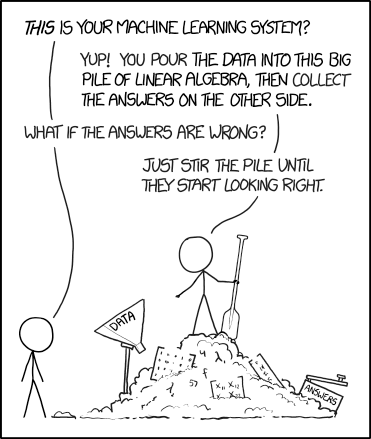
\includegraphics[height=50mm]{figures/machine_learning.png}

% Title, author and degree
\vspace{1.0cm}
{\FontLb (Deep) Generative Models for Multi-Variate Time-Series} \\ % <<<<< EDIT TITLE
%\vspace{0.2cm}
%{\FontMn Subtitle (optional)} \\
%\vspace{1.9cm}
\vspace{2.6cm}
{\FontMb Guilherme P. Grijó Pires} \\ % <<<<< EDIT NAME
\vspace{2.0cm}
{\FontSn \coverThesis} \\
\vspace{0.3cm}
{\FontLb Electrical and Computer Engineering} \\ % <<<<< EDIT COURSE
\vspace{1.0cm}
{\FontSn %
\begin{tabular}{ll}
 \coverSupervisors: & Prof. Mário Alexandre Teles de Figueiredo \\ % <<<<< EDIT NAME
\end{tabular} } \\
\vspace{1.0cm}
{\FontMb \coverExaminationCommittee} \\
\vspace{0.3cm}
{\FontSn %
\begin{tabular}{c}
\coverChairperson:     Prof. Full Name          \\ % <<<<< EDIT NAME
\coverSupervisor:      Prof. Full Name 1 (or 2) \\ % <<<<< EDIT NAME
\coverMemberCommittee: Prof. Full Name 3           % <<<<< EDIT NAME
\end{tabular} } \\
\vspace{1.5cm}
{\FontMb Month Year} \\ % <<<<< EDIT DATE (corresponds to date of oral examination)
%
\end{center}

 % file "Thesis_FrontCover.tex"
\cleardoublepage

% ----------------------------------------------------------------------
% Quote page (optional)
% ----------------------------------------------------------------------
\null\vskip5cm%
\begin{flushright}
    \textit{What I cannot create, I do not understand.}\\
     - Richard Feynman
\end{flushright}
\vfill\newpage

 % file "Thesis_Quote.tex"
\cleardoublepage

% ----------------------------------------------------------------------
%  Acknowledgments (optional)
% ----------------------------------------------------------------------
\section*{\acknowledgments}

% Add entry in the table of contents as section
\addcontentsline{toc}{section}{\acknowledgments}

A few words about the university, financial support, research advisor, dissertation readers, faculty or other professors, lab mates, other friends and family...

 % file "Thesis_Acknowledgements.tex"
\cleardoublepage

% ----------------------------------------------------------------------
%  Abstract (both in English and Portuguese)
% ----------------------------------------------------------------------
\section*{Resumo}

% Add entry in the table of contents as section
\addcontentsline{toc}{section}{Resumo}

Inserir o resumo em Portugu\^{e}s aqui com o máximo de 250 palavras e acompanhado de 4 a 6 palavras-chave...

\vfill

\textbf{\Large Palavras-chave:} palavra-chave1, palavra-chave2,...

   % file "Thesis_Resumo.tex"
\cleardoublepage

\section*{Abstract}

% Add entry in the table of contents as section
\addcontentsline{toc}{section}{Abstract}


\vfill

\textbf{\Large Keywords:} 
 % file "Thesis_Abstract.tex"
\cleardoublepage

% ----------------------------------------------------------------------
%  Table of contents, list of tables, list of figures and nomenclature
% ----------------------------------------------------------------------

% Table of contents
%
\tableofcontents
\cleardoublepage 

% List of tables
%
% Add entry in the table of contents as section
\phantomsection
\addcontentsline{toc}{section}{\listtablename}
% Generate list
\listoftables
\cleardoublepage 

% List of figures
%
% Add entry in the table of contents as section
\phantomsection
\addcontentsline{toc}{section}{\listfigurename}
% Generate list
\listoffigures
\cleardoublepage 

% Nomenclature
%
% entries of nomenclature list
% The definitions can be placed anywhere in the document body
% and their order is sorted by <symbol> automatically when
% calling makeindex in the makefile
%
% The \glossary command has the following syntax:
%
% \glossary{entry}
%
% The \nomenclature command has the following syntax:
%
% \nomenclature[<prefix>]{<symbol>}{<description>}
%
% where <prefix> is used for fine tuning the sort order,
% <symbol> is the symbol to be described, and <description> is
% the actual description.

% ----------------------------------------------------------------------
% Roman symbols [r]
\nomenclature[ru]{$\bf u$}{Velocity vector.}
\nomenclature[ru]{$u,v,w$}{Velocity Cartesian components.}
\nomenclature[rp]{$p$}{Pressure.}
\nomenclature[rC]{$C_D$}{Coefficient of drag.}
\nomenclature[rC]{$C_L$}{Coefficient of lift.}
\nomenclature[rC]{$C_M$}{Coefficient of moment.}

% ----------------------------------------------------------------------
% Greek symbols [g]
\nomenclature[g]{$\rho$}{Density.}
\nomenclature[g]{$\alpha$}{Angle of attack.}
\nomenclature[g]{$\beta$}{Angle of side-slip.}
\nomenclature[g]{$\mu$}{Molecular viscosity coefficient.}
\nomenclature[g]{$\kappa$}{Thermal conductivity coefficient.}

% ----------------------------------------------------------------------
% Subscripts [s]
\nomenclature[s]{$x,y,z$}{Cartesian components.}
\nomenclature[s]{$i,j,k$}{Computational indexes.}
\nomenclature[s]{$\infty$}{Free-stream condition.}
\nomenclature[s]{ref}{Reference condition.}
\nomenclature[s]{$n$}{Normal component.}

% ----------------------------------------------------------------------
% Supercripts [t]
\nomenclature[t]{T}{Transpose.}
\nomenclature[t]{*}{Adjoint.}

 % file "Thesis_Nomenclature.tex"
%
% Add entry in the table of contents as section
\phantomsection
\addcontentsline{toc}{section}{\nomname}
% Insert glossary/nomenclature section produced by MakeIndex
\printnomenclature
\cleardoublepage

% entries of glossary list

% The definitions can be placed anywhere in the document body
% and their order is sorted by <symbol> automatically when
% calling makeindex in the makefile
%
% The \glossary command has the following syntax:
%
% \glossary{entry}
%
% The \nomenclature command has the following syntax:
%
% \nomenclature[<prefix>]{<symbol>}{<description>}
%
% where <prefix> is used for fine tuning the sort order,
% <symbol> is the symbol to be described, and <description> is
% the actual description.

% ----------------------------------------------------------------------

\glossary{name={\textbf{MDO}},description={Multi-Disciplinar Optimization is an engineering technique that uses optimization methods to solve design problems incorporating two or more disciplines.}}

\glossary{name={\textbf{CFD}},description={Computational Fluid Dynamics is a branch of fluid mechanics that uses numerical methods and algorithms to solve problems that involve fluid flows.}}

\glossary{name={\textbf{CSM}},description={Computational Structural Mechanics is a branch of structure mechanics that uses numerical methods and algorithms to perform the analysis of structures and its components.}}

 % file "Thesis_Glossary.tex"

% Add entry in the table of contents as section
\phantomsection
\addcontentsline{toc}{section}{\glossaryname}
% Insert glossary section produced by MakeIndex
\printglossary
\cleardoublepage

% Set arabic numbering (1,2,...) after preface
%
\setcounter{page}{1}
\pagenumbering{arabic}

% ----------------------------------------------------------------------
%  Chapters
% ----------------------------------------------------------------------

\chapter{Introduction}
\label{chapter:introduction}

Insert your chapter material here...

%%%%%%%%%%%%%%%%%%%%%%%%%%%%%%%%%%%%%%%%%%%%%%%%%%%%%%%%%%%%%%%%%%%%%%%%
\section{Motivation}
\label{section:motivation}

Relevance of the subject...


%%%%%%%%%%%%%%%%%%%%%%%%%%%%%%%%%%%%%%%%%%%%%%%%%%%%%%%%%%%%%%%%%%%%%%%%
\section{Topic Overview}
\label{section:overview}

Provide an overview of the topic to be studied...


%%%%%%%%%%%%%%%%%%%%%%%%%%%%%%%%%%%%%%%%%%%%%%%%%%%%%%%%%%%%%%%%%%%%%%%%
\section{Objectives}
\label{section:objectives}

Explicitly state the objectives set to be achieved with this thesis...


%%%%%%%%%%%%%%%%%%%%%%%%%%%%%%%%%%%%%%%%%%%%%%%%%%%%%%%%%%%%%%%%%%%%%%%%
\section{Thesis Outline}
\label{section:outline}

Briefly explain the contents of the different chapters...

 % file "Thesis_Introduction.tex"
\cleardoublepage

\chapter{Probabilistic Modelling}
\label{chapter:probmodel}

\section{Introduction}
\label{section:probmodelintro}
Probabilistic modelling is a set of techniques that leverage probability
distributions and random variables to posit, test and refine hypothesis about
the behaviour of systems. Given observations of a system, the task of probabilistic
modelling normally boils down to finding a probability distribution which:
\begin{itemize}
    \item Is consistent with the observed data;
    \item Is consistent with \textbf{new}, previously unobserved data, originated\
        in the same system.
\end{itemize}

This probability distribution is commonly called the \emph{model}. A good model
will be a good \emph{emulator} of the true generative process that originated
the observed data. In loose terms, this can be summarized as:
\begin{align}
    \mbox{data} \sim p(\mbox{data}|\mbox{hypothesis}^*),
\end{align} where $\text{hypothesis}^*$ is the optimal hypothesis.

Via Bayes' Law, we can write:
\begin{align}
    p(\mbox{hypothesis}|\mbox{data}) = \frac{p(\mbox{data}|\mbox{hypothesis})p(\mbox{hypothesis})}{p(\mbox{data})}
\end{align}

In practice, a modeller will search for an hypothesis that maximizes (some form,
or approximation of) this expression. For simpler problems, this search happens
in closed-form, i.e., there is an expression to compute the optimal hypothesis,
given data. However, for most real-world problems there is no closed-form solution,
and the modeller has to resort to algorithms and approximations, and will only
be able to find \textbf{local} optima for the above expression, in most cases.

It's also worth noting that there are effectively infinite candidate distributions -
each one an hypothesis for how the system at hand generates data. It is common
to make use of domain knowledge and assume the true system has a certain intrinsic
structure and form, and to use these assumptions to constrain the space of
candidate hypothesis. Assumptions about structure usually translate to conditional
independence claims between some or all of the observed variables; assumptions
about form translate into the use of specific parametric families to govern some
or all of the observed variables. These assumptions are commonly connected between
themselves (for example, when conjugate likelihood-prior pairs are used).

When parametric forms are used, an hypothesis is uniquely defined by the set of
parameters it requires - commonly called $\theta$\footnote{For the type of models
and problems dealt with in this work, I will assume $\theta$ is finite, but it's
worth noting that there are models for which the size of $\theta$ \emph{grows}
with the dataset size. These are called non-parametric models. They come with
their own advantages and disadvantages, which are out of the scope of this work.}.

\section{Model Complexity}
\label{section:modelcomplexity}
Intuitively, the size of $\theta$ is deeply connected with the expressiveness
of the distribution. In practice, this translates to the observation that if we
make the model\footnote{Throughout this work I will be using the words \emph{model}
and \emph{distribution} almost interchangeably, making it clear when context isn't
enough.} expressive enough, it can fit the observed data arbitrarily well. Naïvely,
this would be a desirable characteristic to exploit - it's always possible to increase
the likelihood by adding parameters to the model. However, increasing model
complexity normally comes at the expense of generalization. This phenomenon is
commonly referred to as \emph{overfitting}, and there are several
angles from which to explain it and interpret it. Namely:
\begin{itemize}
    \item The classical perspective is that of the bias-variance tradeoff. To
        understand this, consider the concept of an Hypothesis Class - a set
        of hypotheses in which, via some procedure, the modeller will search
        for an hypothesis that is consistent with the observed data, and is
        expected to generalize to unseen data. Said procedure is what is normally
        referred to as \emph{fitting} the model to the data. In the case of
        parametric models, the set of models of a given parametric form, with
        a parameter-vector of a certain fixed size, is an example of an Hypothesis
        Class. Intuitively, a more complex Hypothesis Class is more likely to
        contain the true hypothesis (or a good approximation to it). However,
        the more complex the Hypothesis Class, the larger the search-space -
        the higher the number of candidate hypothesis. In this sense, an increase
        in the size of the search-space often translates into an increase of the
        sensitivity to the problem variables (in the case of learning and inference,
        this means sensitivity to initialization and to the data used to fit).
        Conversely, a simpler model will constitute a smaller search-space, hence
        the search procedure will be less sensitive to initalization and problem
        variables. However, the true hypothesis (or a good approximation to it)
        is less likely to be contained in it - precisely because it is a smaller
        Hypothesis Class. The bias-variance tradeoff is a summary of these observations:
        a highly complex model is potentially able to achieve a low expected error
        on observed data (low bias), but will tend to be extremely sensible to small
        variations on its input (high variance). Conversely, a simpler model will
        be more robust to variations on its input (low variance), but won't have the same
        modelling capacity and will produce a larger expected error (high bias). %\footnote{
        %The number of parameters is far from being the best measure of complexity
        %of a model. Nevertheless, it is a good proxy to compare model complexity
        %between models of the same parametric family. However, recent work by
        %Belkin et al. \cite{Belkin2018Dec} shows that modern machine learning
        %contexts, in which the number of parameters is far larger than in classical
        %settings, have to be understood under a measure of model complexity
        %different than the traditional ones. This is because it is now common
        %practice to fit highly overparameterized models to a point of interpolation
        %(close to zero training error), still being able to achieve good generalization.
        %To explain this, the authors of \cite{Belkin2018Dec} 
        %}
    \item Andrey Kolmogorov's and Gregory Chaitin's ideas on Algorithmic Information
        Theory \cite{chaitin-leibniz}, and Kolmogorov complexity  are another
        useful lens through which to regard this question. Consider that data are
        measurements of phenomena. Modelling is concerned with finding the
        laws that explain/govern these phenomena. Intuitively, if the laws are
        as complex as the data they intend to explain, they aren't explaining anything.
        AIT formalizes this notion by borrowing the concept of \emph{program} to
        define the generative process by which observed data comes to existence.
        The complexity of a dataset is then easy to define: it is the size of
        the \textbf{smallest}\footnote{Note the emphasis on "smallest" - this is
        because any program can be made arbitrarily redundant, and thus arbitrarily large.}
        program that generates the observed data. And the appropriate unit with
        which to measure the size of a program - and, as we've now seen, the
        complexity of a dataset - is bits\footnote{Or the basic unit of memory
        of the computer where the data generating program would run}. The parallel
        between these ideas and the question of overfitting is thus easy to make:
        a program (or a model and its parameter vector)  is useful if it 
        \emph{compresses} the data, intuitively because to do so it leverages the
        patterns therein, which are the object of interest in the modelling task.
\end{itemize}

Both of these lines of reasoning make clear that there is a certain balance
in complexity that a good model has to achieve: it should be parsimonious enough
that it won't overfit, but flexible enough that it is able to properly explain
the observed data.  There are strategies to make this mathematically objective.
Some of those methods are the Bayesian Information Criterion, the Akaike
Information Criterion and the Minimum Description Length.

\section{Structure and Latent Variables}
\label{section:probmodellatvar}
In some cases, one might want to leverage some available domain knowledge. This
often translates into assuming that there is some latent structure in the data.
This structure is encoded into latent variables and their influence over the
observable variables.

In this scenario, we become interested in the distribution given by
$p(x, z, \theta_x, \theta_z)$, where $z$ is the latent variable, $\theta_x$ is
the parameter vector for the distribution over $\mathcal{X}$, and $\theta_z$ is
the parameter vector for the distribution over $\mathcal{Z}$.

For structure and latent variables to be useful we normally make the additional
assumption that we have the ability of factorizing that distribution in ways that
make it tractable. If we have a dataset $\mathbf{X} = {x_1, x_2, x_3, ..., x_N}$, with
$N$ i.i.d. samples, and $N$ latent variables, $\mathbf{Z} = {z_1, z_2, z_3, ..., z_N}$,
one common factorization is:
\begin{align}
    p(\mathbf{X}, \mathbf{Z}, \theta) = \Big(\prod^N_{i=1} p(x_i| z_i, \theta_x) p(z_i | \theta_z)\Big) p(\theta_x) p(\theta_z). \label{eq:latentvariable}
\end{align}

It's also possible that the samples of $\mathbf{X}$ have some sort of causal
relation, for instance if they occur ordered in time. In this case, they are not i.i.d.
One way to encode this assumption is to posit an \emph{autoregressive} model, i.e.,
a model in which a random variable depends on the variables that come before it.
If each random variable depends solely on the random variable that precedes it,
this is called a Markov Model. A common variation of the Markov Model is the
Hidden Markov Model, where the autoregressive part of the model is present only
in the latent variables:
\begin{align}
    p(\mathbf{X}, \mathbf{Z}, \theta) = p(z_1) \Big(\prod^N_{i=2} p(x_i | z_i, \theta_x) p(z_i| z_{i-1}, \theta_z) \Big) p(\theta_x) p(\theta_z).
\end{align}

These are merely examples of models with different structure assumptions encoded
into them. Normally, if the structure has a certain regularity, it's possible
to exploit it to obtain tractable (approximate) inference and estimation methods.

\section{Mixture Models}
Mixture Models are a subset of the structure "family" described in \ref{eq:latentvariable},
and they have a central role in this work.

In a Mixture Model there is a discrete latent variable $z_i$ which selects
one of $K$ components from which an observation $x_i$ will be sampled. This
can be summarized as:
\begin{align}
    z_i \sim p(z_i | \pi) \\
    x_i \sim p(x_i | z_i)
\end{align}

It's common to assume that all of the $K$ components are part of the same
parametric family. In that case, we can rewrite the above as:
\begin{align}
    z_i \sim p(z_i | \pi) \\
    x_i \sim p(x_i | \theta_{z_i}),
\end{align} where it is made evident that the discrete variable $z_i$ is selecting
the \textbf{parameter vector} to be used for sample $x_i$.

The most discussed mixture model is the Gaussian Mixture Model, in which the $K$
components of the model are Gaussian distributions.

\section{Approximate Inference}
\label{section:probmodelinf}
Take the expression $p(x, z, \theta)$. For simplicity, let us consider $\theta$
as part of the latent variables $z$. This means that the model is simply written
as the joint distribution: $p(x, z)$. \emph{Inference}\footnote{If we hadn't collapsed
$\theta$ into $z$ and were instead handling separately, we would call \textbf{inference}
to the task of finding $z$ and \textbf{learning} to the task of finding $\theta$}
is the task of finding the most probable $z$ after having observed $x$ . Specifically,
the goal is to find the posterior distribution of $z$, given $x$, i.e.: $p(z|x)$.

Recall Bayes' Law:

\begin{align}
    p(z|x) &= \frac{p(x|z)p(z)}{p(x)} \\
           &= \frac{p(x|z)p(z)}{\int p(x|z')p(z') dz'}
\end{align}

For the vast majority of cases, the integral on the denominator will be
intractable. To overcome this difficulty we normal resort to two families
of methods: Monte-Carlo methods, and Variational methods.

\subsection{Monte-Carlo Methods}
\label{subsection:mcmc}

Monte-Carlo methods work by using sampling techniques to approximate the
intractable integral. The most powerful subclass of these methods is called
Markov-chain Monte-Carlo. Its approach consists of devising a scheme that
allows for sampling from a distribution close to the one of interest. It
accomplishes this by defining a Markov-Chain whose transition function 
is guaranteed to make it converge asymptotically to the distribution of interest,
given some constraints (ergodicity...) (TODO: explain more)

\subsection{Variational Methods}
\label{subsection:variational}
Variational methods work by turning the problem of integration into one of
optimization. They propose a family of parametric distributions, and then
optimize the parameters so as to minimize the "distance" between the approximate
(normally called "variational") distribution and the distribution of interest.

There are two ways to derive the most commonly used objective function for
this problem, which will be detailed in the two following subsections.

\subsubsection{Kullback-Leibler Divergence}
\label{subsubsection:kldiv}

The Kullback-Leibler divergence is a measure\footnote{Note that the KL divergence
isn't symmetric and as such I haven't called it a \emph{metric}} of the distance
between two probability distributions $p$, and $q$. It is given by:

\begin{align}
    KL(q||p) = \int q \log\frac{q}{p}
\end{align}

In the setting of inference, $p$ is the posterior $p(z|x)$ and $q$ is a distribution
in some parametric family, with parameters $\phi$, i.e., $q(z; \phi)$. However,
it's clear that we can't compute the Kullback-Leibler directly, because it
requires the knowledge of both the distributions, and finding $p(z|x)$ is precisely
the task at hand. Let us expand the KL divergence expression:

\begin{align}
    KL(q||p) &= \int q(z) (\log q(x) - \log p(z|x)) dz \\
             &= \int q(z) (\log q(z) - (\log p(x, z) - \log p(x))) dz \\
             &= \mathbb{E}_q [\log q(z)] - \mathbb{E}_q [\log p(x, z)] + \mathbb{E}_q [\log p(x)] \\
             &= \mathbb{E}_q [\log q(z)] - \mathbb{E}_q [\log p(x, z)] + \log p(x) \\
\end{align}

The last term is constant w.r.t $q(z)$. In that sense, for a fixed $p(x)$,
minimizing the KL divergence is equivalent to minimizing
\begin{align}
    \mathbb{E}_q [\log q(z)] - \mathbb{E}_q [\log p(x, z)],
\end{align} which is equivalent to maximizing
\begin{align}
    \mathbb{E}_q [\log p(x, z)] - \mathbb{E}_q [\log q(z)]. \label{eq:elbokldiv}
\end{align} This quantity is commonly refered to as ELBO - Expectation Lower BOund.
It can be rewritten as:

\begin{align}
    ELBO(q) &= \mathbb{E}_q [\log p(x, z)] - \mathbb{E}_q [\log q(z)] \\
            &= \mathbb{E}_q [\log p(x|z)] + \mathbb{E}_q [\log p(z)] - \mathbb{E}_q [\log q(z)]
\end{align}

In this form, each term of the ELBO has an easily interpretable role:
\begin{itemize}
    \item $\mathbb{E}_q [\log p(x|z)]$ tries to maximize the conditional likelihood of $x$. That
        can be seen as assigning high probability mass to values of $z$ that \emph{explain} $x$
        well.
    \item $\mathbb{E}_q [\log p(z)]$ is the symmetric of the crossentropy between
        $q(z)$ and $p(z)$. Maximizing this quantity is equivalent of minimizing
        that crossentropy. This can be regarded as a regularizer that discourages
        $q(z)$ of being too different from the prior $p(z)$.
    \item $ - \mathbb{E}_q [\log q(z)]$ is the entropy of $q(z)$. Maximizing
        this term incentivizes the probability mass of $q(z)$ to be spread out:
        another form of regularization.
\end{itemize}

\subsubsection{A lower bound on $\log p(x)$}
\label{subsubsection:elbo}

Another way of approaching the intractable posterior is to start by stating
that our inherent goal is to maximize $p(x)$, or equivalently $\log p(x)$. Given
that, consider the following:
\begin{align}
    \log p(x) &= \log \int p(x, z) dz\\
    &= \log \int q(z) \frac{p(x, z)}{q(z)} dz \\
    &= \log \mathbb{E}_q[\frac{p(x, z)}{q(z)}] \label{eq:elbojensen1} \\
    &\geq \mathbb{E}_q[\log \frac{p(x, z)}{q(z)}] \label{eq:elbojensen2} \\
    &\geq \mathbb{E}_q[\log p(x, z)] - \mathbb{E}_q[q(z)] \label{eq:elbojensen3}
\end{align}

To understand this derivation, consider Jensen's inequality, given (in one of
its forms) by:
\begin{align}
    \phi(\mathbb{E}[X]) \leq \mathbb{E}[\phi(X)], \label{eq:jensen}
\end{align} where $\phi(.)$ is a convex function.

If $\xi(.)$ is a concave function, then $- \xi(.)$ is a convex function, and we
obtain the reverse inequality (substituting $\phi(.)$ with $-\xi(.)$ in the
inequality in \ref{eq:jensen}):
\begin{align}
    -\xi(\mathbb{E}[X]) &\leq \mathbb{E}[-\xi(X)] \\
    \xi(\mathbb{E}[X]) &\geq \mathbb{E}[\xi(X)]
\end{align}

This form is the most useful for us, since $\log$ is a concave function. Using
this, the step between \ref{eq:elbojensen1} and \ref{eq:elbojensen2} is made
obvious.

Note that the right-hand side of \ref{eq:elbojensen3} is the same quantity
we arrived at in \ref{eq:elbokldiv}, and that it is a lower-bound on the
quantity we want to maximize, and so we want to maximize it. It's worth noting
that when $q(z) = p(z|x)$, the bound is tight.

\cleardoublepage

%\input{MixtureModels}
%\cleardoublepage

\chapter{Normalizing Flows}
\label{chapter:probmodel}

\section{Introduction}
The best known and studied probability distributions are rarely expressive
enough for real-world datasets. However, they have properties that make them
amenable to work with, for instance: tractable parameter estimation and closed-form
likelihood functions.

As has been described, one way to obtain more expressive models is to assume the
existence of latent variables, leverage certain factorization structures, and to
use well-known distributions for the individual factors of the product that
constitutes the model's joint distribution. By using these structures and choosing
specific combinations of distributions (namely, conjugate prior-likelihood pairs),
these models are able to stay tractable - normally via bespoke estimation/inference/learning
algorithms.

%Structures are easily encoded by Probabilistic Graphical Models, which are a
%framework to easily express conditional independence assumptions and to specify
%complex probabilistic models.

Another approach to obtaining expressive probabilistic models is to apply
transformations to a simple distribution, and use the Change of Variables
formula to compute probabilities in the transformed space. This is the basis
of Normalizing Flows, an approach proposed by \author{shakir_nf} in \cite{shakir_nf},
and which has since evolved and developed into the basis of multiple SoA techniques
for density estimation [TODO: cite examples here].

\section{Change of Variables}
Given a probability distribution $p(z)$, with probability density function $f_Z(.)$,
and a bijective and continuous function $g$, it's possible to write an expression
for the probability density function $f_Y(.)$ of the random variable $y$ that is
obtained by applying $g$ to samples of $p(z)$:
\begin{align}
    \mbox{if } z &\sim p(z) \\
    \mbox{and } y &= g(z) \\
    \mbox{then } f_Y(y) &= f_Z(g^{-1}(y))\Big|\det\Big(\frac{d}{dy}g^{-1}(y)\Big)\Big|
\end{align}

For this to be useful, some objects have to be easily computable:
\begin{itemize}
    \item $f_Z(z)$ - the starting distribution's probability density function.
        It is assumed that there is a closed-form expression to compute this. In
        practice, this is normally one of the basic distributions (Gaussian,
        Uniform, etc.)
    \item $\det\Big(\frac{d}{dy}g^{-1}(y)\Big)$ - the determinant  of the Jacobian
        matrix of $g^{-1}(.)$ . For most transformations this is not "cheap" to compute.
        As will be shown, the main challenge of Normalizing Flows is to find
        transformations that are expressive and for which 
        the determinants of their Jacobian matrices are "cheap" to compute.
\end{itemize}

\section{Normalizing Flows}
Let us have $L$ transformations $h_\ell$ that fulfill the above two points, and
let $z_\ell$ be the result of applying transformation $h_{\ell-1}$, with the
exception of $z_0$, which is obtained by sampling from $p(z_0)$, the base distribution.
Furthermore, let $g$ be the composition of the $L$ transformations.

Applying the Change of Variables formula:
\begin{align}
    \mbox{if } z_0 &\sim p(z_0) \\
    \mbox{and } y &= h_L \circ h_{L-1} \circ ... \circ h_0(z_0) \\
    \mbox{then } f_Y(y) &= f_Z(g^{-1}(y))\Big|\det\Big(\frac{d}{dy}g^{-1}(y)\Big)\Big| \\
                        &= f_Z(g^{-1}(y))\prod_{\ell=1}^{L}\Big|\det\Big(\frac{d}{dz_{\ell+1}}h_{\ell}^{-1}(z_{\ell+1})\Big)\Big| \\
                        &= f_Z(g^{-1}(y))\prod_{\ell=1}^{L}\Big|\det\Big(\frac{d}{dz_{\ell}}h_{\ell}\Big(h_{\ell}^{-1}(z_{\ell+1}\Big)\Big)\Big|^{-1} \label{eq:nflowderivation}
\end{align}

Replacing $h_{\ell}^{-1}(z_{\ell+1}) = z_\ell$ in \ref{eq:nflowderivation}:

\begin{align}
         f_Y(y) &= f_Z(g^{-1}(y))\prod_{\ell=1}^{L}\Big|\det\Big(\frac{d}{dz_{\ell}}h_{\ell}\Big(z_\ell)\Big)\Big)\Big|^{-1} \\
    \log f_Y(y) &= \log f_Z(g^{-1}(y)) - \sum_{\ell=1}^{L} \log \Big|\det\Big(\frac{d}{dz_{\ell}}h_{\ell}(z_\ell)\Big) \Big| \label{eq:nflowsfinal}
\end{align}

Depending on the task, one might prefer to replace the second term in \ref{eq:nflowsfinal}
with a sum of log-abs-determinants of the Jacobians of the inverse transformations.
This switch would imply replacing the minus sign before the sum with a plus sign:
\begin{align}
    \log f_Y(y) &= \log f_Z(g^{-1}(y)) + \sum_{\ell=0}^{L-1} \log \Big|\det\Big(\frac{d}{dz_{\ell+1}}h_{\ell}^{-1}(z_{\ell+1})\Big) \Big|
\end{align}


\section{Flow examples}
In the Normalizing Flows literature, a Flow is the name given to each of the
individual transformations that are composed to form a Normalizing Flow.

\section{Real NVP}



\cleardoublepage

\chapter{Variational Mixture of Normalizing Flows}
\label{chapter:vmonf}

\section{Introduction}

Lorem ipsem Lorem ipsemLorem ipsemLorem ipsemLorem ipsem
Lorem ipsemLorem ipsemLorem ipsemLorem ipsemLorem ipsemLorem ipsem
Lorem ipsemLorem ipsemLorem ipsemLorem ipsem
Lorem ipsemLorem ipsemLorem ipsemLorem ipsemLorem ipsem
Lorem ipsemLorem ipsemLorem ipsemLorem ipsemLorem ipsem

\cleardoublepage

\chapter{Conclusions}
\label{chapter:conclusions}

Insert your chapter material here...


% ----------------------------------------------------------------------
\section{Achievements}
\label{section:achievements}

The major achievements of the present work...


% ----------------------------------------------------------------------
\section{Future Work}
\label{section:future}

A few ideas for future work...

 % file "Thesis_Conclusions.tex"
\cleardoublepage

% ----------------------------------------------------------------------
%  Bibliography
% ----------------------------------------------------------------------

% Add entry in the table of contents as chapter
\phantomsection
\addcontentsline{toc}{chapter}{\bibname}

% Include all references in .bib file, even non-cited ones...
%\nocite{*} % this should be used carefully because it is not correct!

% Produces the bibliography section when processed by BibTeX
%
% Bibliography style
% > entries ordered alphabetically
%\bibliographystyle{plain}
% > unsorted with entries appearing in the order in which the citations appear.
%\bibliographystyle{unsrt}
% > entries ordered alphabetically, with first names and names of journals and months abbreviated
%\bibliographystyle{abbrv}
% > entries ordered alphabetically, with reference markers based on authors' initials and publication year
%\bibliographystyle{alpha}
%
% Replacement bibliography styles provided by 'natbib' package
% (plainnat.bst, abbrvnat.bst, unsrtnat.bst )
% > entries ordered alphabetically
%\bibliographystyle{plainnat}
% > unsorted with entries appearing in the order in which the citations appear.
%\bibliographystyle{unsrtnat}
% > entries ordered alphabetically, with first names and names of journals and months abbreviated
%\bibliographystyle{abbrvnat} % <<<<< SELECT IF USING REFERENCES BY AUTHOR/YEAR
% > entries ordered alphabetically, with reference markers based on authors' initials and publication year
%\bibliographystyle{alpha}
%
% Custom bibliography style adapted from 'natbib' package
%   (based on http://tex.stackexchange.com/questions/5053/is-it-possible-to-get-unsrt-abbrv-bibliography)
%   (unsrtnat.bst + abbrvnat.bst -> abbrvunsrtnat.bst)
%   (original files copied from:
%   http://tug.ctan.org/macros/latex/contrib/natbib/abbrvnat.bst
%   http://tug.ctan.org/macros/latex/contrib/natbib/unsrtnat.bst
% > unsorted with entries appearing in the order in which the citations appear, with first names and names of journals and months abbreviated.
\bibliographystyle{abbrvunsrtnat} % <<<<< SELECT IF USING REFERENCES BY NUMBER (CITATION ORDER)

% External bibliography database file in the BibTeX format
\bibliography{Thesis_bib_DB} % file "Thesis_bib_DB.bib"

\cleardoublepage

% ----------------------------------------------------------------------
%  Appendix (optional)
%
%  CAUTION: 1) the main document (up to the conclusions) shall not exceed 80 pages
%           2) the document shall not exceed a total of 100 pages (per IST regulations)
% ----------------------------------------------------------------------
%\appendix

% add page number prefix according to apendix chapter (optional)
%\renewcommand{\thepage}{\thechapter.\arabic{page}}

% re-set arabic numbering (A.1,A.2,...) (optional, use only if chapter prefix is added)
%\setcounter{page}{1}

%\chapter{Vector calculus}
\label{chapter:appendixVectors}

In case an appendix if deemed necessary, the document cannot exceed a total of 100 pages...

Some definitions and vector identities are listed in the section below.

% ----------------------------------------------------------------------
\section{Vector identities}
\label{section:vectorIdentities}

\begin{equation}
	\nabla \times \left( \nabla \phi \right) = 0
	\label{eq:cross_nnp}
\end{equation}

\begin{equation}
	\nabla \cdot \left( \nabla \times {\bf u} \right) = 0
	\label{eq:dotCross_nnu}
\end{equation}

 % file "Thesis_Appendix_A.tex"
%\cleardoublepage

% ----------------------------------------------------------------------
\end{document}
% ----------------------------------------------------------------------

